
%%
%% This .tex file is for use with BibLaTeX.
%%
%% As of Spring 2023, the School of Graduate Studies requires some minimum accessibility requirements for all electronic theses. Accessibility is difficult to produce with LaTeX on the front end, but fortunately it is quite easy to meet the requirements on the back end using Adobe (not Adobe Reader). Simply download the PDF of your thesis and follow this guide: https://case.edu/gradstudies/sites/case.edu.gradstudies/files/2023-02/CWRU%20Thesis%20and%20Dissertation%20Accessiblity%20Guide_0.pdf
%%%%%%%%%%%%

\documentclass[12pt]{cwru_thesis}
\usepackage[hyphens]{url}
\usepackage{indentfirst}
\usepackage{lipsum}
\usepackage{tabularx}
\usepackage{graphicx}
\usepackage{hyperref}
\hypersetup{colorlinks=true, linkcolor=black, filecolor=black, urlcolor=black, citecolor=black}
\urlstyle{same}
% \usepackage[acronym,toc]{glossaries}
\usepackage[intoc]{nomencl}
\renewcommand{\nomname}{List of Symbols}

\usepackage{mathptmx}
\usepackage[T1]{fontenc}
\usepackage[utf8]{inputenc}
\usepackage{amsfonts, amsmath, amsthm, amssymb}


\newcommand{\dif}{\mathrm{d}}
\newcommand{\Dif}{\mathrm{D}}
\renewcommand{\vec}[1]{\ensuremath{\underline{#1}}}
\newcommand{\grad}{\underline{\nabla}}
\newcommand{\curl}{\underline{\nabla} \times}
\newcommand{\lap}{\underline{\nabla}^2}
\renewcommand{\div}{\underline{\nabla} \cdot}
\newcommand{\paren}[1]{\left( {#1} \right)}
\newcommand{\norm}[1]{\lVert#1\rVert}

% Must use biblatex to produce the Published Contents and Contributions, per-chapter bibliography (if desired), etc.
\usepackage[style=authoryear, sorting=none, citestyle=authoryear-comp]{biblatex}
% Name of your .bib file(s)
\addbibresource{example.bib}



% \makeglossaries
%%%%%%%%%%%%%%%%%%%%%%%%%%%%%%%%%%%%%%%%%%%%%%%%%%%%%%%%%%%%%%%%%%%%%%%%%%%%%%%%%%%%%%%
%Glossary entries


%Acronyms to include in the list of acronyms
% \newacronym{mda}{MDA}{Multipath Discovery Algorithm}
% \newacronym{mca}{MCA}{Multipath Classification Algorithm}

\begin{document}
\pagenumbering{roman}

% Do remember to remove the square brackets!
\title{A Topographical Evaluation of Load Balancers} %Title of your thesis in title case
\author{Omar Loudghiri} %Your name

\degreeaward{Master's of Science in Computer Science}                 % Degree to be awarded
\department{Department of Computer Science and Data Science}
\university{Case Western Reserve University}    % Institution name  
\unilogo{cwru_logo.eps}                                 % Institution logo
\defendmonth{August, 2024}          % Graduation month and year
\defenddate{July 10th, 2024}          % Date of thesis defense

%Committee Member names. If you have a different number of committee members for your defense, you will need to edit lines 183-190 of cwru_thesis.cls accordingly.
\committeeChair{An Wang} %Committee Chair's name
\committeeOne{Mark Allman} %Committee member #1's name
\committeeTwo{Vincenzo Liberatore} %Committee member #2's name
\committeeThree{Mehmet Koyuturk} %Committee member #3's name

%%  If you'd like to add the CWRU logo from your title page, simply add the "[logo]" text to the maketitle command. Note that the School of Graduate Studies doesn't like this.
\maketitle

\begin{dedication} 	 
  TBD
\end{dedication}

\begin{KeepFromToc}
  \tableofcontents
\end{KeepFromToc}
\listoftables
\listoffigures



\begin{acknowledgements}
   TBD
\end{acknowledgements}

%If you have acroynms you wish to define, include this line. If not, you may delete it. See https://www.overleaf.com/learn/latex/Glossaries#Acronyms for more information about how to use Acronyms.

% \printglossary[type=\acronymtype, title=List of Abbreviations]

%If you have terms you wish to define in a glossary, include this line. If not, you may delete it. See https://www.overleaf.com/learn/latex/Glossaries for more information about how to use Glossaries
% \printglossary

%If you have a nomenclature section for defining symbols, include this line. If not, you may delete it. See https://www.overleaf.com/learn/latex/Nomenclatures for more information about how to use Nomenclatures
\printnomenclature

\begin{abstract}
This thesis examines the prevalence and characteristics of load balancing on the Internet. Using data collected daily from November 2023 to April 2024, we analyzed web traffic to understand load balancing behavior and its impact on network performance.\\

Measurements were conducted using Paris Traceroute with the Multipath Detection Algorithm (MDA). Our findings show that 82.2\% of paths in the Top-2000 dataset and 62.5\% in the Rand-2000 dataset contain load balancers.\\

Load balancers exhibited dynamic behavior, with frequent changes and an average presence duration of about a month in the Top-2000 dataset and about two weeks in the Rand-2000 dataset. We also explored Layer 3 load balancing, focusing on Cisco Express Forwarding (CEF), noting both its efficiency and drawbacks.\\

Our study provides insights into the structure and dynamics of load balancing across the Internet. Future work includes expanding the number of destinations, adapting advanced algorithms for better load balancer detection, and developing tools to improve identification accuracy.
\end{abstract}


\mainmatter

\setcounter{secnumdepth}{2}

\chapter{Introduction} 
\label{chap:intro}

\section{Introduction to Load Balancing}

Networks are crucial to the Internet we rely on today by enabling communication, commerce, and data exchange on a global scale. These networks are constructed through an interconnected array of user devices, routers, and servers. Understanding the architecture and dynamics of these networks is vital for enhancing their efficiency and reliability. Research has long focused on mapping and analyzing network structures to improve their performance and resilience \textbf{[\cite{paxson_endtoend96}]}.

A key aspect of network optimization is load balancing, a practice employed by network operators to manage traffic distribution and scale network capacity. By distributing traffic across multiple servers or network paths, load balancing ensures that no single server becomes overwhelmed, promoting both efficiency and reliability. It is essential to maintain a current understanding of both network structures and load balancing techniques to sustain robust and efficient network operations \textbf{[\cite{10371400}]}.

Load balancing is a network management technique that distributes traffic across multiple servers or network paths. A load balancer is a piece of network equipment that can direct packets to one of several available routes, anticipating that each route will yield a similar result. This distribution helps prevent any single server from becoming overwhelmed and ensures efficient use of network resources \textbf{[\cite{f52023loadbalancing}]}.

Originally developed as network-based hardware, load balancing now often functions within routers \textbf{[\cite{bourke2001server}]}. It plays a crucial role in modern infrastructure by ensuring high availability, scalability, security, and performance. Applications today must handle millions of simultaneous sessions, and load balancers dynamically distribute this traffic across servers with duplicate data, ensuring reliable and fast data delivery. This process can also provide redundancy. If a server fails, traffic may be redirected to maintain continuous access. However, it is important to note that while load balancers can provide redundancy, this is not always the case. If the load balancer itself fails and it is not part of a redundant setup, it can become a single point of failure.

Load balancing has several benefits, including enhancing security by potentially minimizing attack surfaces and rerouting traffic if a server is compromised. By distributing traffic, load balancers reduce the risk of a single server being targeted and overwhelmed by an attack. An attack surface refers to the number of entry points through which an attacker can try to enter or extract data from a system. With load balancing, the exposure of any single server is minimized, thereby reducing the overall attack surface. However, for the security benefits to be effective, the load balancer itself must be secure and properly configured \textbf{[\cite{10.1145/3098593.3098595}]}.

Additionally, load balancing optimizes performance by managing resource use and handling traffic spikes. Various algorithms, such as round-robin and least connections, help distribute traffic based on real-time conditions. This ensures that all servers share the load equally and prevents any single server from becoming a bottleneck, thereby maintaining smooth and efficient operation of the network \textbf{[\cite{8316818}]}.\\

\section{Project Motivation and Goals}

The primary motivation for this project is to quantify the prevalence and characteristics of load balancing in the Internet. By measuring load balancing behavior and mapping the presence of load balancers across commonly used paths, this research aims to enhance our understanding of their impact. This includes identifying and categorizing load balancers, analyzing their deployment, and understanding the resulting network paths and their implications for the broader Internet infrastructure.

Understanding how load balancing affects network performance and reliability is crucial for developing more efficient and resilient network systems. Effective load balancing can prevent single points of failure, manage high traffic volumes, and ensure continuous service availability. By studying current load balancing practices and their outcomes, we can identify areas for improvement and develop strategies to enhance network stability and efficiency. This research will contribute to a better understanding of the critical role load balancing plays in maintaining the robustness and efficiency of the Internet.





\section{Areas of Study}

In the following chapters, we explore several aspects of web traffic and network optimization. We begin by discussing related work in Chapter 2. This chapter covers essential tools and methodologies such as Traceroute, the Multipath Detection Algorithm (MDA), Paris Traceroute, and Scamper, including their features and applications in detecting and classifying load balancers in the Internet.

In Chapter 3, we provide an overview of our research methodology. This includes background information on datasets like the Alexa Top 1 Million Websites and the Team Cymru IP to ASN list. We detail our approach to discovering load balancers, including measurement frequency, and IP list compilation.

Chapter 4 examines the topography of load balancers. We analyze the distribution of load balancers using our datasets, and compare insights from these datasets. We also delve into the analysis of next hops after load balancers, identifying Autonomous Systems with the most next hops, and exploring changes over time.

In Chapter 5, we study Layer 3 load balancing, focusing on network layer load balancing and Cisco Express Forwarding (CEF). We also discuss modifications to the MDA algorithm and the challenges and future work associated with enhanced probing trials.










\chapter{Related Works}

Traceroute is a network diagnostic tool used to track the path packets take from one IP address to another. It works by sending packets with gradually increasing time-to-live (TTL) values. Each router along the path decreases the TTL of the packet by one. When the TTL reaches zero, the router sends back an error message to the sender, revealing its IP address. This process is repeated with incrementing TTL values, allowing Traceroute to map out the entire route to the destination.

Traceroute provides insights into the structure and behavior of the network by identifying each hop along the route. However, traditional Traceroute may not handle load-balanced paths well, as it can be misled by the varying paths packets may take. To address this, Paris Traceroute and MDA are used to obtain more accurate measurements by maintaining consistent flow identifiers, thus avoiding misinterpretation caused by load balancers.

\section{Paris Traceroute}
In \textbf{[\cite{4261334}]}, the authors present an enhanced version of Traceroute to indentify load balancers along with a comprehensive study on load-balanced paths, highlighting the significance of recognizing load balancing in contemporary networking by demonstrating how it affects traffic distribution and path diversity. 

In their second paper \textbf{[\cite{augustin2010measuring}]}, which aimed to measure the presence of load balancers in the Internet by conducting measurements from 15 sources to over 68,000 destinations, their study reveals that the traditional single-path concept no longer holds. They found that the routes to 39\% of the destinations traversed a load balancer. Some of their results suggest up to 72\% when considering different types of load balancing. While the specifics of these different types of load balancing are out of scope for this project, our goal is to update the community's understanding of the topology of load balancers almost 10 years after their paper.


This study was significant in showing the prevalence of load balancers. The insights gained from this work are critical for developing more realistic network models and improving the design and reliability of Internet applications.



\section{Multipath Detection Algorithm (MDA)}

The Multipath Detection Algorithm (MDA) is a key component of Paris Traceroute, designed to identify and trace multiple load-balanced paths between a source and a destination. Traditional Traceroute tools often fail to detect load balancing because they assume a single path. In contrast, MDA systematically discovers all paths by varying flow identifiers in probe packets.

The MDA operates hop-by-hop, sending probes to identify all interfaces at each hop. For a given interface \(r\) at hop \(h-1\), MDA generates several flow identifiers to ensure probes reach \(r\). Flow identifiers are unique markers within packet headers, such as combinations of source and destination IP addresses, port numbers, and protocol types . It then sends these probes one hop further to discover the next-hop interfaces \(s_1, s_2, \ldots, s_n\).

To determine the number of probes \(k\) needed to discover all paths with a high degree of confidence, MDA assumes \(r\) is part of a load balancer that splits traffic evenly across \(n\) paths. If fewer than \(n\) interfaces are found, MDA stops. Otherwise, it increases \(n\) and sends additional probes to test the hypothesis.

To identify whether a load balancer uses per-packet or per-flow balancing, MDA sends probes with a constant flow identifier. If responses come from multiple interfaces, it indicates per-packet balancing. If all responses come from the same interface, it suggests per-flow balancing. MDA uses statistical methods to ensure a high level of confidence (typically 95\%) in its classification.

Per-flow balancing means that all packets within the same flow (i.e., packets sharing the same source and destination IP addresses, port numbers, and protocol) follow the same path through the network. This ensures that packets arrive in order, which is crucial for the correct reassembly and processing of data streams.

Per-packet balancing, on the other hand, distributes individual packets across multiple paths. While this can maximize the use of available network resources, it can lead to packet reordering since packets from the same flow might take different paths and arrive out of order. This can complicate the reassembly process and potentially impact the performance of applications sensitive to packet order.


For instance, to reject the hypothesis of \(n = 2\) with 95\% confidence, MDA sends \(k = 6\) probes. If load balancing across up to 16 interfaces is suspected, MDA may send up to \(k = 96\) probes to ensure all paths are discovered. This process allows MDA to effectively enumerate all paths and classify the type of load balancing in use.


The paper by \textbf{[\cite{4261334}]} is one of the few studies that actively measures the presence and behavior of load balancers in the Internet. Although their work provides a strong foundation, further investigation is needed to account for the evolving nature of Internet infrastructure and load balancing techniques.

By leveraging Paris Traceroute and MDA, we conduct extensive measurements to map the global distribution of load balancers and analyze their impact on network performance and reliability.


\section{Scamper}

Scamper, presented in \textbf{[\cite{luckie2010scamper}]}, is a versatile tool used for conducting large-scale Internet measurements. It was easily modified to support more fine-tuned measurements using the Multipath Detection Algorithm (MDA), enhancing its capability to identify and analyze load-balanced paths.



\subsection{Multipath Detection Algorithm (MDA) in Scamper}

Scamper implements the Multipath Detection Algorithm (MDA) described by Augustin et al. to infer all interfaces visited between a source and destination in a per-flow load-balanced Internet path. MDA achieves this by deliberately varying the flow identifier that a router may compute when load balancing. Probes with different flow identifiers may take different paths, thereby revealing different parts of the forward IP path.

In addition to the ICMP and UDP methods originally implemented by Augustin et al., which vary the ICMP checksum and UDP destination port values, Scamper implements a UDP method that varies the source port instead of the destination port. This prevents the probes from appearing as a port scan and enables probing past firewalls that block UDP probes to ports above the usual range used by Traceroute. Scamper also implements TCP methods that vary the flow identifier by changing either the source or destination port, depending on the user’s choice.

Scamper's MDA Traceroute functionality was used to conduct scheduled data collection throughout this project.

\section{Multipath Classification Algorithm (MCA)}

Recent advances in network technology and the adoption of IPv6 have enabled more complex load balancing strategies. \textbf{[\cite{9155387}]} introduced the Multipath Classification Algorithm (MCA), which enhances the existing Multipath Detection Algorithm (MDA). While MDA systematically varies probes' flow identifiers to identify load-balanced paths, MCA extends this by considering arbitrary combinations of bits in the packet header for load balancing.

The key contributions of MCA include enhanced classification and comprehensive measurements. MCA identifies the specific bits in the packet header used by load balancers, providing a more detailed and accurate classification than MDA. Additionally, MCA characterizes load balancing on both IPv4 and IPv6 Internet paths, showing that load balancing is more prevalent and sophisticated than previously reported.


Despite these advancements, using MCA was not feasible for our research due to its higher complexity and longer runtime. MCA's improvements come at the cost of increased probing time and complexity, making it less practical for large-scale measurements.\\



While MCA offers improvements in identifying and classifying load balancers, it is less accessible for fine-tuning and practical use. For our research, we opted to use MDA due to its better integrability with existing tools (scamper) and faster runtime performance in order to conduct daily measurments. MDA's established methodologies and ease of implementation make it a more practical choice for large-scale measurements. 
 

\chapter{Methodology}

This chapter details the methods used to collect data for detecting and characterizing load balancers in network paths. We employed two lists derived from the Alexa Top 1 Million Websites list and performed Paris Traceroute measurements to these hostnames. The collected data was then processed to identify load balancers and analyze their behavior.

\section{Data Sources and Selection Criteria}

To ensure the feasibility of daily measurements, pilot measurements were conducted, which indicated that approximately 2000 hostnames could be processed per day. This constraint informed our selection of two distinct subsets from the Alexa list, enabling daily measurements while managing logistical constraints.

The Alexa Top 1 Million Websites list was used to obtain hostnames for this research. A current version of the Alexa list was obtained when we started our data collection in November 2023. The Alexa list is widely used in network measurement studies due to its popularity, since it is not known for high accuracy for ranks below 100,000 sites \textbf{[\cite{alexa2023top1m}]}, only the top 100,000 is in consideration.

For our study, we selected two distinct subsets from the Alexa list:
\begin{itemize}
    \item \textbf{Top-2000 List:} This list includes the top 2000 domains from the Alexa list, designed to cover the most used websites on the Internet, ensuring that the analysis captures the behavior and infrastructure of significant routes.
    \item \textbf{Rand-2000 List:} This list comprises 2000 random domains selected from the top 100,000 websites on the Alexa list, with a new random selection made each time we ran the measurement. This aims to provide a well-rounded analysis of the Internet's topology by including popular but not exclusively top-ranked sites. This random list excludes the top-2000 hostnames from the previous list.
\end{itemize}

\section{Discovering Load Balancers}

We recorded the paths between our vantage point and a set of popular hosts to detect and characterize load balancers along these paths. 

\subsection{Measurement Frequency and Timeline}
\label{subsec:freq}


To ensure the feasibility of daily measurements, 2000 hostnames were chosen for the Paris Traceroute process. Each hostname takes an average of 40 seconds to return a complete trace with load balancer information. This duration allows the script to run through 2000 hostnames in approximately 23 hours, making it possible to conduct measurements on a daily basis.

The goal of daily measurements is to assess trends and variations in load balancing behavior over time. To maintain feasibility, we ran measurements in parallel for the Top-2000 list and the Rand-2000 list each day. Each measurement started at 5 am EST and ran in Alexa rank order for Top-2000 and in the random order the list was created in Rand-2000. After completing the measurements, there was a one-hour buffer before the next run began at 5 am the following day.

The measurements were run continuously from December 1, 2023, to April 16, 2024, on a Linux machine at the International Computer Science Institute (ICSI) in Berkeley, CA. Some pilot measurements were also run beforehand from both machines at ICSI and at CWRU.
This timeline ensured the collection of extensive data over several months, capturing potential variations and trends in load balancing behavior and network topology over time. 

Using the top 2000 websites allows us to measure load balancers on sites that are heavily accessed, providing insights into the infrastructure of widely used services. The random selection of 2000 sites from the top 100,000 ensures a broader view of the Internet's topology, capturing data from a diverse set of sites.



\section{Team Cymru IP to ASN List}

An Autonomous System (AS) is a collection of IP networks and routers under the control of a single organization that presents a common routing policy to the internet. Each AS is assigned a unique identifier known as an Autonomous System Number (ASN), which facilitates the routing of data between different ASes. ASes play a critical role in the overall structure of the internet, as they help manage the flow of data, ensuring efficient and reliable connectivity across various networks. They are often managed by internet service providers (ISPs), large enterprises, or educational and government institutions.

To map routers to organizations in our analysis, we used the Team Cymru IP to ASN mapping service to resolve IP addresses to their corresponding Autonomous System Numbers (ASNs). Team Cymru maps IP numbers to BGP prefixes and ASNs using data from over 50 BGP feeds, updated every four hours \textbf{[\cite{teamcymru2023ipasn}]}.\\  


 
 We collected ASN-to-IPv4 address information from Team Cymru every month, with their permission. This list was used to cross-reference the IPs identified as load balancers, their next hops, and their destination IPs, providing detailed insights into the load balancers discovered. Table \ref{tab:bgp_asn_info} shows the fields we obtain for each IP address, detailing data about  the Autonomous System it belongs to. 

\begin{table}[h]
    \centering
    \begin{tabular}{|l|l|}
        \hline
        \textbf{Field} & \textbf{Example} \\
        \hline
        BGP Origin ASN & 23489 \\
        \hline
        BGP Peer ASN & 199.88.100.1 \\
        \hline
        BGP Prefix & 199.88.100.0/24 \\
        \hline
        Prefix Country Code (assigned) & US \\
        \hline
        Prefix Registry (assigned) & arin \\
        \hline
        Prefix Allocation Date & 1994-03-28 \\
        \hline
        ASN Country Code (assigned) & US \\
        \hline
        ASN Registry (assigned) & arin \\
        \hline
        ASN Allocation Date & 1994-03-28 \\
        \hline
        ASN Description & MARINK12, US \\
        \hline
    \end{tabular}
    \caption{BGP and ASN Information from team Cymru data}
    \label{tab:bgp_asn_info}
\end{table}




For each domain in the Rand-2000 and Top-2000 lists, the Paris Traceroute tool was used with the Multipath Detection Algorithm (MDA) to conduct Traceroute measurements. The IP to ASN mapping service was then used to resolve IP addresses to their corresponding Autonomous System Numbers (ASNs). This information was used to cross-reference the IPs identified as load balancers, their next hops, and their destination IPs.

\section{Ethical Considerations}

This research adhered to strict ethical standards to ensure no harm was caused during data collection. We performed active measurements with care, ensuring they did not overflood the network. We ran only the two necessary probes in parallel to prevent any network disruptions.

No personal information was collected in our data. We ensured that our data collection methods did not cause any disruptions. Ethical considerations were carefully followed based on the recommendations in \textbf{[\cite{partridge2016ethical}]}



\chapter{Topography of Load Balancers}

In this chapter, we examine the distribution and prevalence of load balancers across two different datasets resulting from two distinct lists: the Top-2000 and the Rand-2000. By analyzing these datasets, we aim to understand how load balancers are utilized in the infrastructure of popular and randomly selected websites.

\section{Analysis of Load Balancer Distribution}

This section examines the distribution of load balancers in out datasets by looking at paths that have at least one load balancer when accessing a domain. To provide a clearer picture of global usage, we also exclude entries related to UCB,US, which reflect local network conditions. 

\subsection{Top-2000 Dataset}

The Top-2000 dataset consists of 117 days of data collected between November 9, 2023, and April 16, 2024. During this period, the number of domains with at least one load balancer ranged from a minimum of 279 to a maximum of 1680. The average number of domains with load balancers was 1644.08, indicating that 82.2\% of the paths to these top domains include load balancers. The median value of 1668 further supports the observation that the majority of these domains consistently use load balancers.

The minimum of 279, along with the lower bound outliers, are usually due to measurement interruptions either caused by hardware issues or by an error or timeout that was not caught by our error checking. We made sure to adjust our code as the measurements went on to make it more reliable.

When we exclude UCB,US data, which accounts for local network dependencies and may not be representative of the entire internet, we see a different picture. The adjusted dataset without UCB,US shows that the number of domains with at least one load balancer ranges from 81 to 1482, with an average of 1439.03 and a median of 1463. This indicates that 71.9\% of the paths to these top domains include load balancers when excluding local network influences.

\subsection{Rand-2000 Dataset}

The Rand-2000 dataset includes 112 days of data collected over the same period, from November 9, 2023, to April 16, 2024. The number of domains with at least one load balancer in this dataset varied between 1205 and 1297. The average number of domains with load balancers was 1251.29, with a median of 1252. These statistics show that 62.5\% of the paths to these randomly selected domains include load balancers, indicating a substantial use of load balancers across a diverse set of websites.

When excluding UCB,US data, the Rand-2000 dataset shows that the number of domains with at least one load balancer ranges from 994 to 1094, with an average of 1046.27 and a median of 1046. This shows that 52.3\% of the paths to these randomly selected domains include load balancers when excluding local network influences.

\subsection{Comparison and Insights}

The plot in Figure \ref{fig:stat_plot} illustrates the number of domains with at least one load balancer over time for both the Top-2000 and Rand-2000 datasets, including the adjusted data excluding UCB,US. This visual representation shows that the number of detected load balancers is relatively constant over the measurement period.

\begin{figure}[h]
\centering
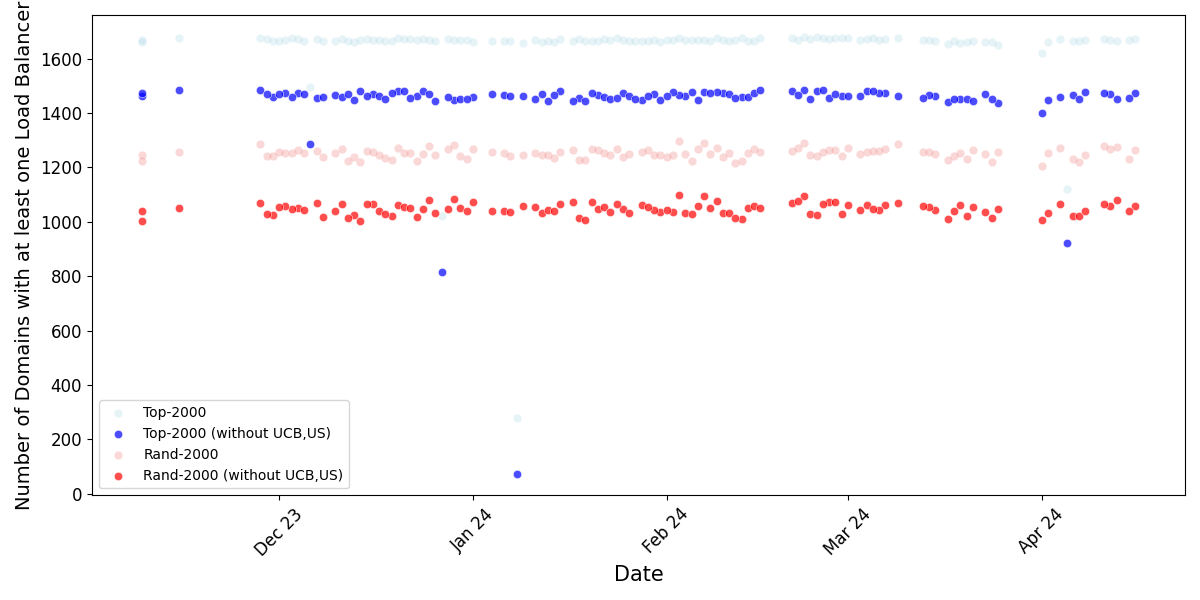
\includegraphics[width=\textwidth]{figures/scatter_plot_domains.png}
\caption{Number of Domains with at least one Load Balancer Over Time}
\label{fig:stat_plot}
\end{figure}

Counting UCB,US would not make sense as that is dependent on our local network, and not all local networks have load balancers. Hence, we need to show the representation considering the local network and not considering the local network to illustrate the difference. 

The higher average and median values in the Top-2000 dataset are indicate the higher usage of load balancers in managing traffic for the most visited websites. These sites likely experience higher and more variable traffic, necessitating robust load balancing solutions to ensure uptime and performance. Meanwhile, the Rand-2000 dataset demonstrates that load balancing is also prevalent for a broad range of domains. Excluding UCB,US data, we see a more accurate representation of load balancer usage that is independent of local network influences.

The plot clearly shows two trends: one with the influence of the local network and one without. The light colors represent the original data, while the dark colors show the adjusted data excluding UCB,US. This is to put our data in context and not let our local netwrok bias the image we are getting of the global network. 


While it is important to isolate local load balancers when evaluating the global picture, the UCB load balancers will still be considered in the following sections unless otherwise noted. Their behavior still provides valuable insights into the general workings of load balancers.
\newpage

\section{Analysis of Next Hops After Load Balancers}

We focused on understanding the behavior of next hops after load balancers. This analysis helps us gain insights into how load distribution is managed.

\subsection{Top-2000 Dataset}

The Top-2000 dataset consists of 192,357 load balancers. The analysis reveals that the number of next hops after a load balancer ranges from a minimum of 2 to a maximum of 102. The average number of next hops is approximately 3.90, indicating a moderate level of load distribution across multiple paths. The median value stands at 3.0, suggesting that half of the load balancers have either three or two next hops. The standard deviation is 5.75, which means a significant variability in the number of next hops. Furthermore, the 75th percentile is at 5.0, while the 95th percentile reaches 13.0, showing that a small number of load balancers have a very high number of next hops (\>15).

\subsection{Rand-2000 Dataset}

In comparison, the Rand-2000 dataset includes 140,144 load balancers. Here, the number of next hops ranges from a minimum of 2 to a maximum of 25. The average number of next hops is 2.58, indicating a higher level of load distribution compared to the Top-2000 dataset. The median number of next hops is 2, suggesting that more than half of the load balancers have only two next hops. The standard deviation is 1.34, indicating lower variability. The 75th percentile is 2.0, and the 95th percentile is 3.0. This shows that most load balancers in this dataset are less complex compared to those in the Top-2000 dataset. They primarily have only 2 or 3 next hops, with some outliers having up to 25, but the general majority are simple 2-3 next hop load balancers.

\begin{figure}[h]
    \centering
    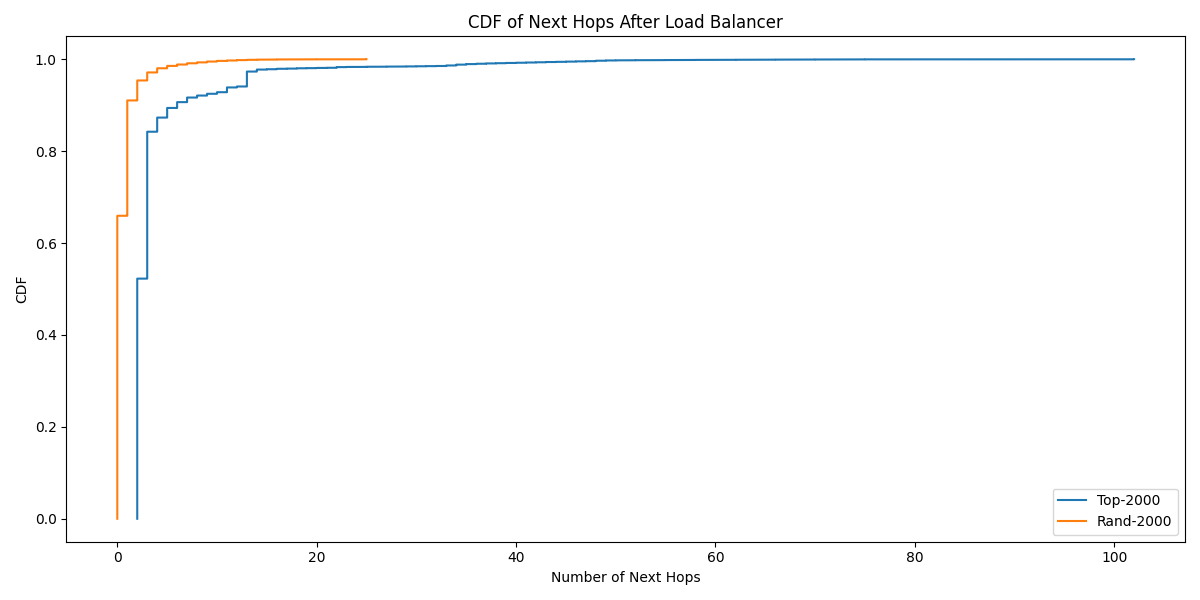
\includegraphics[width=\linewidth]{figures/cdf_next_hops.png}
    \caption{CDF of Next Hops After Load Balancers for Top-2000 and Rand-2000 Datasets}
    \label{fig:cdf_next_hops}
\end{figure}

Figure \ref{fig:cdf_next_hops} illustrates the cumulative distribution function (CDF) of the number of next hops after load balancers for both the Top-2000 and Rand-2000 datasets. The CDF provides a visual representation of the distribution and helps in comparing the two datasets. As shown, the Top-2000 dataset demonstrates a wider spread with more load balancers having a higher number of next hops, whereas the Rand-2000 dataset shows a more concentrated distribution with most load balancers having fewer next hops.



The differences in the number of next hops between the two datasets highlight the varying network configurations and load distribution strategies. The higher variability in the Top-2000 dataset suggests a more complex and distributed network structure, indicating the need for more expansive infrastructure due to the higher traffic these sites receive. In contrast, the Rand-2000 dataset's lower variability and fewer next hops suggest a simpler network configuration for less commonly used paths. These findings align with our hypothesis that the most visited websites require more extensive load balancing to manage their significant traffic demands.

\section{Analysis of ASes with Most Next Hops}

The analysis of Autonomous Systems (ASes) with the highest average number of next hops reveals significant insights into the infrastructure and load balancing requirements of these networks. 
The ASes with the most next hops typically indicate a robust infrastructure with a greater need for load balancing. This could be due to a high volume of traffic, requiring efficient distribution across multiple servers to avoid bottlenecks, or due to specific requirements such as traffic filtering based on the source. Table \ref{tab:as_next_hops} shows the ASes that own the load balancers with the most next hops accross both datasets.\\

\begin{table}[h!]
    \centering
    \begin{tabularx}{\textwidth}{|X|r|}
        \hline
        \multicolumn{2}{|c|}{\textbf{Top 10 ASes by Average Number of Next Hops (Top-2000)}} \\
        \hline
        \textbf{AS} & \textbf{Average Next Hops} \\
        \hline
        ORACLE-BMC-31898, US & 90.69 \\
        FACEBOOK, US & 24.97 \\
        GOOGLE, US& 24.16 \\
        ADJUST-, DE & 20.59 \\
        CHINA169-BJ China Unicom Beijing , CN & 19.82 \\
        CHINANET-BJ-AP, China Telecommunications, CN & 15.44 \\
        CLOUDFLARENET, US & 13.95 \\
        ALIBABA-CN-NET Alibaba Advertising , Ltd., CN & 13.89 \\
        CHINANET-SCIDC-AS-AP CHINANET SiChuan, CN & 13.82 \\
        CHINANET-BACKBONE No.31, Jin-rong Street, CN & 13.74 \\
        \hline
        \multicolumn{2}{|c|}{\textbf{Top 10 ASes by Average Number of Next Hops (Rand-2000)}} \\
        \hline
        \textbf{AS} & \textbf{Average Next Hops} \\
        \hline
        ORACLE-BMC-31898, US & 23.03 \\
        FACEBOOK, US & 7.88 \\
        CHINA169-BJ China Unicom Beijing, CN  & 6.78 \\
        CHINANET-SH-AP China Telecom Group, CN & 5.20 \\
        ADJUST-, DE& 4.36 \\
        CHINANET-SCIDC-AS-AP CHINANET SiChuan, CN & 3.25 \\
        CT-IDC No.287, Jin-rong Street, CN  & 2.95 \\
        CHINANET-BACKBONE No.31, Jin-rong Street, CN & 2.78 \\
        CT-HANGZHOU-IDC No.288, Fu-chun Road, CN & 2.28 \\
        CHINANET-BJ-AP, China Telecommunications, CN & 2.20 \\
        \hline
    \end{tabularx}
    \caption{Top 10 ASes by Average Number of Next Hops for Top-2000 and Rand-2000}
    \label{tab:as_next_hops}
\end{table}

The order of ASes is about the same across both datasets, indicating that larger ASes with more budget tend to develop their infrastructure and add many next hops to their load balancers. This means that even if an AS already has a lot of infrastructure, it remains prevalent even in the less popular paths.

We see a significant presence of Chinese load balancers. According to Bhaskar et al. \textbf{[\cite{bhaskar2021}]}, some Chinese providers use load balancers to enforce censorship, which explains their prevalence. Their study found that packet headers, such as source IP address and source port, can influence DNS censorship. They discovered that 37\% of IPs across 56\% of ASes showed changes in censorship behavior based on these parameters. This means that Chinese load balancers are used not only for load distribution but also to control access to information, demonstrating their dual role in managing traffic and enforcing censorship.

In the Rand-2000 dataset, the top 7 to 10 ASes have an average number of next hops below three. Since the minimum is two, these numbers aren't as significant, indicating that most load balancers in this range are of similar rank and complexity.

Despite the similarities in the order of ASes, the Top-2000 dataset shows higher numbers of next hops due to the higher average usage and need for more extensive load balancing. This underscores the importance of expansive infrastructure for the most visited websites, which require robust load balancing solutions to manage their significant traffic demands.

\newpage
\section{Overall Analysis of Next Hop ASes Matches and Mismatches}

In our comprehensive analysis across all load balancers, we identified significant patterns in the matching and mismatching of next hops.

Our results revealed that out of a total of 192,357 load balancers analyzed in the Top-2000 dataset, and 140,144 load balancers in the Rand-2000 dataset, we observed a total of 104,214 unique load balancers. Among these, 80,979 were fully matching, where every next hop AS matched the load balancer AS, representing 77.7\% of the total unique load balancers. Fully matching next hops indicate that the AS ensures its load balancers are dedicated to managing the load for that specific AS and not for others.


Partially matching next hops, where at least one but not all next hops matched the load balancer AS, accounted for 402 instances, or 0.4\% of the total. These partial matches suggest a mixed routing strategy where some paths are optimized within the AS, while others diverge.
\begin{figure}[h!]
    \centering
    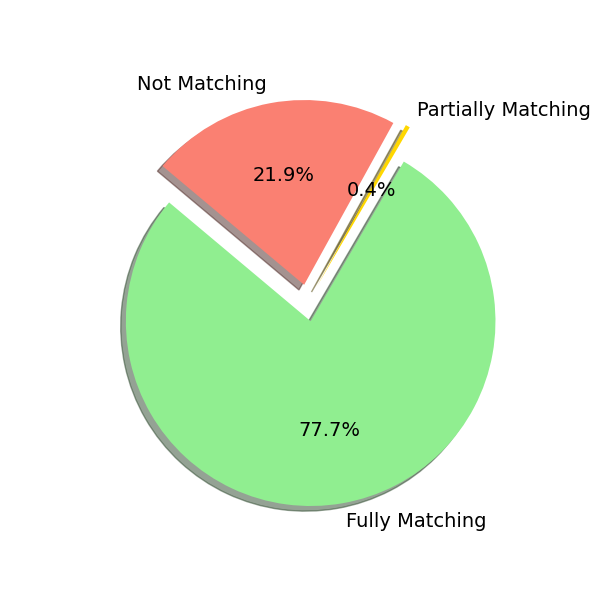
\includegraphics[scale=0.6]{figures/overall_match_mismatch.png}
    \caption{Overall Load Balancer Next Hop Matching}
    \label{fig:overall_match_mismatch}
\end{figure}


Next hops with no matching AS comprised 22,833 instances, making up 21.9\% of the total load balancers. A no match indicates that a service provider is managing and balancing the load of a node that it does not own. This could mean that load balancing is offered as a paid service by that provider. Additionally, it could be that the AS deems it necessary to balance the load for the integrity of the network, especially if the network is directly adjacent to them, as disruptions could occur if there is an overload close to their nodes. It could also be government-mandated, as seen with some Chinese public providers.

Figure~\ref{fig:overall_match_mismatch} illustrates the overall distribution of fully matching, partially matching, and no matching next hops. The pie chart provides a clear visual representation of the dominant patterns in next hop routing behavior.


Our analysis also highlighted the top Autonomous Systems (ASes) based on the number of matches and mismatches. Table \ref{tab:match_no_match} presents the top ASes in each category.

Overall, the findings suggest that while a majority of next hops maintain consistency within their ASes, there are notable instances of partial and no matches. This indicates that ASes mostly perform load balancing for their own nodes rather than for external nodes. This behavior makes sense because load balancing for external nodes would be costly without significant benefits to internal networks. However, the 22.3\% of non-matching load balancers is quite surprising, with some of the reasons it could happen explained above. 


\begin{table}[h!]
    \centering
    \begin{tabular}{|l|r|}
        \hline
        \multicolumn{2}{|c|}{\textbf{Top 10 ASes with Fully Matching Next Hops}} \\
        \hline
        \textbf{AS} & \textbf{Count} \\
        \hline
        UCB, US & 30,890 \\
        Google, US & 13,516 \\
        ChinaNet Backbone No.31, Jin-Rong Street, CN & 6,420 \\
        Comcast-7922, US & 5,460 \\
        China169-BJ China Unicom Beijing Province Network, CN & 4,028 \\
        KDDI Corporation, JP & 3,204 \\
        Facebook, US & 2,321 \\
        Microsoft-Corp-MSN-AS-Block, US & 2,260 \\
        Cogent-174, US & 1,769 \\
        KIXS-AS-KR Korea Telecom, KR & 1,744 \\
        \hline
        \textbf{Total} & 80,979 \\
        \hline
        \multicolumn{2}{|c|}{\textbf{Top 10 ASes with Partially Matching Next Hops}} \\
        \hline
        \textbf{AS} & \textbf{Count} \\
        \hline
        ChinaNet-IDC-BJ-AP IDC, China Telecommunications Corporation, CN & 158 \\
        ChinaNet Backbone No.31, Jin-Rong Street, CN & 125 \\
        RelianceJio-IN Reliance Jio Infocomm Limited, IN & 30 \\
        Yandex, RU & 18 \\
        GlobalDC, FI & 17 \\
        Level3, US & 15 \\
        NL-Gigapop, US & 12 \\
        HiNetUSA HiNet Service Center in U.S.A, TW & 12 \\
        Alibaba-CN-Net Hangzhou Alibaba Advertising Co., Ltd., CN & 4 \\
        Alibaba-CN-Net Alibaba US Technology Co., Ltd., CN & 4 \\
        \hline
        \textbf{Total} & 402 \\
        \hline
        \multicolumn{2}{|c|}{\textbf{Top 10 ASes with No Matching Next Hops}} \\
        \hline
        \textbf{AS} & \textbf{Count} \\
        \hline
        CONE, US & 6,908 \\
        Cogent-174, US & 2,580 \\
        UCB, US & 2,525 \\
        ChinaNet Backbone No.31, Jin-Rong Street, CN & 2,440 \\
        ChinaNet-IDC-BJ-AP IDC, China Telecommunications Corporation, CN & 854 \\
        Level3, US & 849 \\
        Yahoo-1, US & 608 \\
        CSUNET-NE, US & 312 \\
        Google, US & 216 \\
        BTN-ASN, US & 207 \\
        \hline
        \textbf{Total} & 22,833 \\
        \hline
    \end{tabular}
    \caption{Top 10 ASes with Fully Matching, Partially Matching, and No Matching Next Hops}
    \label{tab:match_no_match}
\end{table}


\newpage


UCB, US, is the local Autonomous System, and therefore it is normal to find great amounts of load balancers belonging to it. The presence of UCB, US in the table highlights how load balancing typically works, with the majority of its load balancers managing internal nodes within its network. Although UCB, US appears on the no matching list, the number is significantly lower. This could indicate that it has allocated some load balancers to external nodes, either to minimize their impact on adjacent networks or through agreements with other ASes, such as Internet2, given their academic basis and potential collaboration to maintain network stability.

Another noteworthy AS is CONE, which refers to CyrusOne, one of the largest data center companies in the world. This presence supports the hypothesis that no matching load balancers are being sold as a service to their customers. Similarly, Cogent, a major internet service provider, appears prominently in the list, reinforcing this notion.

While ChinaNet load balancers do show up in the no matching category, they are not the dominant presence there. Instead, ChinaNet is more prevalent in the matching load balancers category. This indicates that, despite their possible role in censorship and strict network controls, ChinaNet primarily uses its load balancers to manage internal network traffic.
\newpage
\section{Change Over Time}

This section presents the statistics for the Top-2000 and Rand-2000 datasets, including the total number of days observed, the average daily changes, and the number of reappearances. Additionally, the top 5 most consistent and least consistent load balancers for both datasets are listed.

\subsection{Top-2000 Dataset}

Over the observation period of 116 days, an average of approximately 253.47 load balancers were added per day in the Top-2000 dataset. Conversely, an average of 251.21 load balancers were lost each day. The dataset also recorded a total of 82,318 reappearances, indicating the number of times load balancers reappeared after having been previously lost. The average duration of presence for a load balancer in this dataset was 31.10 days.

\begin{table}[h!]
    \centering
    \begin{tabular}{|l|l|}
        \hline
        \textbf{Most Consistent Load Balancers} & \textbf{Duration (days)} \\ \hline
        169.229.0.140 : UCB, US & 116 \\ \hline
        137.164.11.94 : CSUNET-NW, US & 116 \\ \hline
        157.240.81.224 : FACEBOOK, US & 116 \\ \hline
        157.240.112.88 : FACEBOOK, US & 116 \\ \hline
        129.134.118.175 : FACEBOOK, US & 116 \\ \hline
    \end{tabular}
    \caption{Top 5 Most Consistent Load Balancers in Top-2000 Dataset}
\end{table}

In contrast, the least consistent load balancers, each appearing for only a single day, are shown in the following table:

\begin{table}[h!]
    \centering
    \begin{tabular}{|l|l|}
        \hline
        \textbf{Least Consistent Load Balancers} & \textbf{Duration (days)} \\ \hline
        202.97.27.181 : CHINANET-BACKBONE, CN & 1 \\ \hline
        203.208.151.181 : SINGTEL-AS-AP, SG & 1 \\ \hline
        203.208.178.185 : SINGTEL-AS-AP, SG & 1 \\ \hline
        203.208.154.45 : SINGTEL-AS-AP, SG & 1 \\ \hline
        203.208.171.9 : SINGTEL-AS-AP, SG & 1 \\ \hline
    \end{tabular}
    \caption{Top 5 Least Consistent Load Balancers in Top-2000 Dataset}
\end{table}

\begin{figure}[h!]
    \centering
    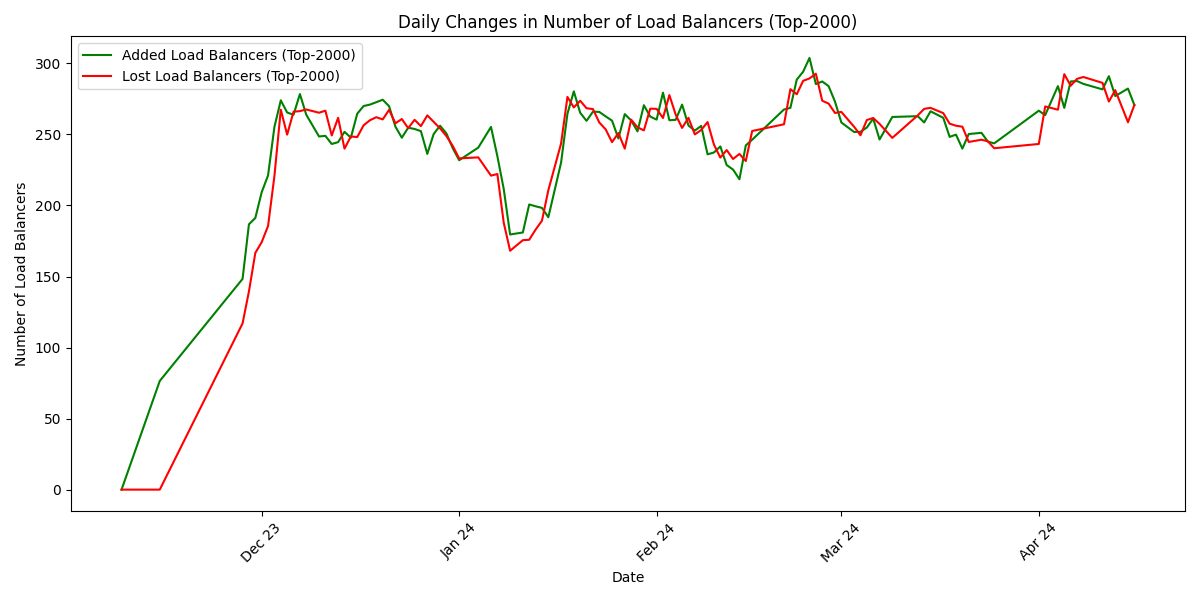
\includegraphics[width=\linewidth]{figures/load_balancer_changes_Top-2000.png}
    \caption{Daily Changes in Number of Load Balancers for Top-2000}
    \label{fig:top2000_changes}
\end{figure}

Figure \ref{fig:top2000_changes} illustrates the dynamic nature of load balancer management in the Top-2000 dataset. The green line represents the number of added load balancers, while the red line represents the number of lost load balancers. The figure shows that while the total number of load balancers remains relatively stable throughout the study period, they are not always the same load balancers. The number of deleted load balancers closely matches the number of new load balancers, indicating a continuous process of adding and removing load balancers to maintain the network's efficiency and performance.

The average duration of presence for a load balancer being 31.10 days indicates that load balancers in the Top-2000 list can be dynamic, often being added when traffic is expected to be more congested. Future work on the presence of load balancers on a more granular hourly basis might reveal whether this dynamic aspect holds true. Such studies could investigate if there is a higher presence of load balancers during peak traffic hours, suggesting that load balancers are actively managed in response to real-time traffic demands.

\newpage

\subsection{Rand-2000 Dataset}

The Rand-2000 dataset, observed over 111 days, provided the following insights: On average, approximately 161.02 load balancers were added per day, while an average of 162.22 load balancers were lost each day. The dataset also recorded a total of 12,139 reappearances, highlighting the instances where load balancers reappeared after being lost. The average duration of presence for a load balancer in this dataset was 12.49 days.

\begin{table}[h!]
    \centering
    \begin{tabular}{|l|l|}
        \hline
        \textbf{Most Consistent Load Balancers} & \textbf{Duration (days)} \\ \hline
        169.229.0.140 : UCB, US & 111 \\ \hline
        137.164.11.94 : CSUNET-NW, US & 41 \\ \hline
        142.251.231.97 : GOOGLE, US & 40 \\ \hline
        142.251.231.99 : GOOGLE, US & 32 \\ \hline
        74.125.50.18 : GOOGLE, US & 30 \\ \hline
    \end{tabular}
    \caption{Top 5 Most Consistent Load Balancers in Rand-2000 Dataset}
\end{table}

The least consistent load balancers in the Rand-2000 dataset, each appearing for a single day, are shown below:

\begin{table}[h!]
    \centering
    \begin{tabular}{|l|l|}
        \hline
        \textbf{Least Consistent Load Balancers} & \textbf{Duration (days)} \\ \hline
        104.44.19.140 : MICROSOFT-CORP-MSN-AS-BLOCK, US & 1 \\ \hline
        104.44.18.166 : MICROSOFT-CORP-MSN-AS-BLOCK, US & 1 \\ \hline
        157.240.51.143 : FACEBOOK, US & 1 \\ \hline
        202.97.53.13 : CHINANET-BACKBONE, CN & 1 \\ \hline
        163.253.2.16 : INTERNET2-RESEARCH-EDU, US & 1 \\ \hline
    \end{tabular}
    \caption{Top 5 Least Consistent Load Balancers in Rand-2000 Dataset}
\end{table}

\begin{figure}[h!]
    \centering
    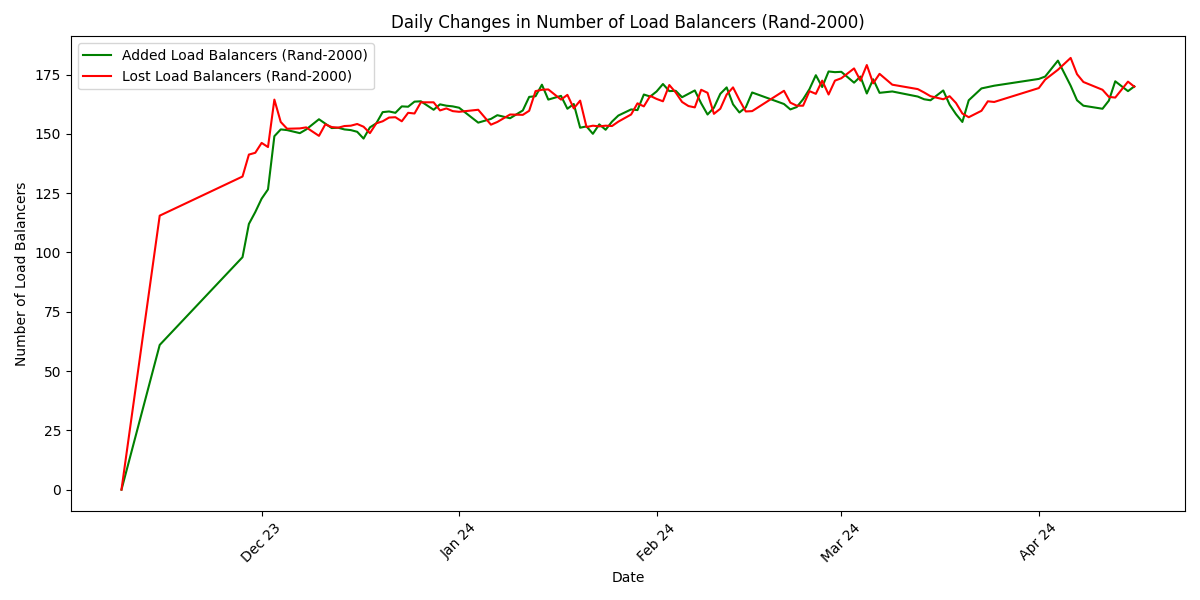
\includegraphics[width=\linewidth]{figures/load_balancer_changes_Rand-2000.png}
    \caption{Daily Changes in Number of Load Balancers for Rand-2000}
    \label{fig:rand2000_changes}
\end{figure}

The analysis shows that load balancers are mostly dynamic and not static, changing over time. The daily change and variability is more evident in the random data because it doesn't consistently target the same paths, leading to higher variability. The average duration of presence further supports this, with load balancers in the Top-2000 dataset averaging 31.10 days, while those in the Rand-2000 dataset average only 12.49 days. 


\subsection{Autonomous Systems}

This subsection presents the AS-specific statistics for both the Top-2000 and Rand-2000 datasets, focusing on daily averages and key metrics related to ASes.

The AS with the most additions per day indicates which AS consistently introduces the most new load balancers. This can reflect the AS's dynamic nature and high level of activity in adjusting its load balancing infrastructure.

The AS with the most removals per day shows which AS frequently removes load balancers. High removal rates can suggest either significant changes in traffic patterns when the load balancing functions are turned off, frequent updates to the network infrastructure when next hops are down, or issues requiring frequent load balancer replacement. It could also be caused by a different route being taken when accessing that website. 

The AS with the longest average duration of presence has load balancers that remain active the longest on average. This indicates a more stable and persistent load balancing infrastructure.

The most consistent AS is present for the most number of times, indicating the AS's load balancers are active across the majority of the observation period, reflecting stability.

The most inconsistent AS is the one that is present for the fewest number of times, suggesting either sporadic use of load balancers or frequent changes in infrastructure. It could also mean that the measurement was a false positive and that it was not truly a load balancer.

The most fluctuating AS has the highest number of load balancer changes, indicating a high level of dynamism in their load balancing strategy, possibly reflecting a need to adapt rapidly to changing traffic conditions or network requirements.

\textbf{Note:} The UCB, US AS was excluded from these statistics as it would consistently be the most reliable AS, given that our tests are conducted from within it.\\

\subsubsection{Top-2000 Dataset}

For the Top-2000 dataset, observed over 116 days:

\begin{itemize}
    \item \textbf{AS with most additions per day:} FACEBOOK, US, Added: 50.34 per day
    \item \textbf{AS with most removals per day:} CSUNET-NW, US, Removed: 50.17 per day
    \item \textbf{AS with longest average duration:} CHINANET-BACKBONE No.31, Jin-rong Street, CN, Average Duration: 159.62 days
    \item \textbf{Most consistent AS:} GOOGLE, US, Present: 75,863 times
    \item \textbf{Most inconsistent AS:} AS-NETIA Warszawa 02-822, PL, Present: 1 time
    \item \textbf{Most fluctuating AS:} CHINANET-BACKBONE No.31, Jin-rong Street, CN, Changes: 11,660 over 116 days
\end{itemize}

\subsubsection{Rand-2000 Dataset}

For the Rand-2000 dataset, observed over 111 days:

\begin{itemize}
    \item \textbf{AS with most additions per day:} CHINANET-BACKBONE No.31, Jin-rong Street, CN, Added: 29.12 per day
    \item \textbf{AS with most removals per day:} FACEBOOK, US, Removed: 29.40 per day
    \item \textbf{AS with longest average duration:} CSUNET-NW, US, Average Duration: 44.09 days
    \item \textbf{Most consistent AS:} GOOGLE, US, Present: 11,153 times
    \item \textbf{Most inconsistent AS:} MTS, RU, Present: 1 time
    \item \textbf{Most fluctuating AS:} CHINANET-BACKBONE No.31, Jin-rong Street, CN, Changes: 6,495 over 111 days
\end{itemize}


The most consistent AS, GOOGLE, US, likely expects a high volume of traffic consistently, necessitating a stable and continuous load balancing infrastructure. In contrast, less consistent ASes, may need to adapt their usage due to the high costs associated with maintaining load balancer infrastructure. This can lead to more sporadic use and frequent changes in infrastructure.

The fact that the same AS, such as GOOGLE, US, is consistent in the Top-2000 dataset but not as consistent in the Rand-2000 dataset suggests deliberate adjustments based on traffic expectations. The Top-2000 list likely experiences more predictable high traffic, requiring continuous load balancing, whereas the Rand-2000 list may see more variable traffic patterns, leading to less consistency.

\newpage



\section{Shared Next Hops Analysis}

This section analyzes the shared next hops between load balancers in both the Top-2000 and Rand-2000 datasets. The objective is to understand the extent to which next hops are shared among multiple load balancers, indicating the presence of common infrastructure and potential load balancing strategies.

\subsection{Top-2000 Dataset}

For the Top-2000 dataset, a total of 9,492 unique next hops were identified. The number of load balancers sharing a next hop ranged from a minimum of 1 to a maximum of 52. On average, each next hop was shared by 5.31 load balancers, with a median value of 2.0. The standard deviation of 6.70 indicates considerable variability in the number of load balancers sharing a next hop. The 75th percentile value was 7.0, and the 95th percentile value was 18.0, showing that a small number of next hops were highly shared among load balancers.

\begin{figure}[h!]
    \centering
    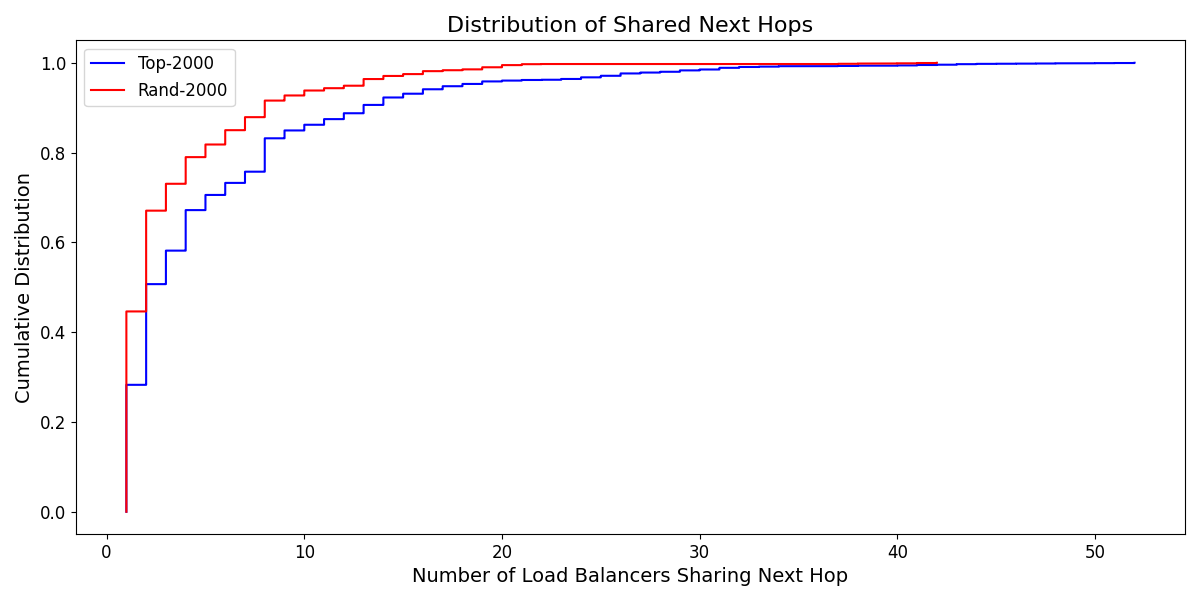
\includegraphics[width=\linewidth]{figures/shared_next_hops_combined.png}
    \caption{Distribution of Shared Next Hops for Top-2000 and Rand-2000}
    \label{fig:shared_next_hops_combined}
\end{figure}

\subsection{Rand-2000 Dataset}

The Rand-2000 dataset revealed 15,797 unique next hops. The number of load balancers sharing a next hop ranged from a minimum of 1 to a maximum of 42. The average number of load balancers sharing a next hop was 3.35, with a median of 2.0. The standard deviation was 4.17, indicating a moderate level of variability. The 75th percentile value was 4.0, and the 95th percentile value was 13.0, suggesting that most next hops were shared by a relatively small number of load balancers.

The analysis of shared next hops between load balancers in both datasets highlights key differences and similarities. The Top-2000 dataset shows a higher average number of load balancers sharing a next hop compared to the Rand-2000 dataset. This suggests that the infrastructure supporting the most popular websites is more interconnected and utilizes shared pathways more frequently than the broader, randomly selected websites.

The distribution of shared next hops, as depicted in Figure~\ref{fig:shared_next_hops_combined}, indicates that while most next hops are shared by a small number of load balancers, there are a few next hops that are highly shared, particularly in the Top-2000 dataset. This can be attributed to the reliance on major network infrastructure providers and common routing paths for high-traffic websites.

Overall, the presence of shared next hops signifies the use of common infrastructure, which can enhance efficiency but also poses risks in terms of single points of failure. The variability in the number of shared next hops across both datasets underscores the complexity and dynamic nature of load balancing in different segments of the Internet.


\chapter{Layer 3 Load Balancing}
In our research, we found many load balancers within the Internet2 Autonomous System. The Internet2 Network was established to support data-intensive research and academic computing needs. Internet2's Looking Glass tool, available for reasearch purposes, allows users to run commands against network devices, enabling some testing and the possibility of viewing active configuration and state information.

The load balancers we found were accessible via the Internet2 looking glass, allowing deeper analysis of their load balancing techniques. We observed that many of the next hops for these load balancers were defined in Cisco Express Forwarding (CEF) tables. The following sections elaborate on the workings of CEF and its role in load balancing.

\section{Network Layer Load Balancing}

Layer 3, known as the network layer, plays a specific role in load balancing by routing packets based on their IP addresses as opposed to considering the current load on the network. This approach focuses on the distribution of traffic across multiple servers without inspecting the packet contents. Unlike higher layers that can make decisions based on the data within the packets, Layer 3 load balancers rely solely on IP addresses and routing tables. This method is efficient and fast but offers less granularity in traffic management, as it does not consider the type or state of the application data. They cannot make decisions based on the content of the traffic, user sessions, or specific application states, which are usually used in more common load balancing strategies. This means that while Layer 3 load balancers can efficiently manage expected large volumes of traffic, they lack detailed and live traffic management capabilities provided by higher-layer solutions \textbf{[\cite{zhang}]}.
Cisco Express Forwarding (CEF) enhance the efficiency of Layer 3 load balancing by pre-computing forwarding information based on previous data on network usage.

\section{Cisco Express Forwarding (CEF)}

Cisco Express Forwarding (CEF)  is a Layer 3 switching technology used to optimize network performance. CEF employs a forwarding information base (FIB) and an adjacency table to expedite the packet forwarding process \textbf{[\cite{cisco2017cef}]}. The following outlines the critical components and operations of CEF:\\

\textbf{Forwarding Information Base (FIB)}: The FIB is used by CEF to make IP destination prefix-based switching decisions. It is conceptually similar to a routing table, maintaining a mirror image of the forwarding information in the IP routing table. When routing or topology changes occur, the IP routing table updates, and these changes are reflected in the FIB. The FIB ensures all known routes are covered, eliminating the need for route cache maintenance.

\textbf{Adjacency Table}: The adjacency table complements the FIB by storing Layer 2 addressing information necessary for packet forwarding. Nodes in the network that can reach each other with a single hop across a link layer have their Layer 2 next-hop addresses stored in this table. 






\subsection{Packet Forwarding Process}

 When a packet arrives, it is placed into input buffers on the receiver hardware component. The Layer 2/Layer 3 forwarding engine accesses the packet's information and determines its route based on the FIB and adjacency table. The appropriate Layer 2 information is then appended to the packet using data from the adjacency table, and the packet is forwarded to its next-hop destination. It also keeps a log of forwarding history to determine future strategies. 




\section{Summary and Findings}


CEF's efficiency in packet forwarding is achieved through its use of optimized data structures (FIB and adjacency tables) and its ability to distribute the forwarding process across different components of the router, particularly in environments where high-speed processing is required. This structured approach allows for fast routing of packets across a network, enhancing overall network performance and scalability. Instead of adjusting in real-time, it determines its expectations of future network behavior by learning from the load history of the system.

The insights gained from analyzing the Internet2 load balancers revealed that most of the next hops for these load balancers are defined within CEF. This means high efficiency and reliability in handling the vast amount of data traffic traversing the Internet2 network. It also means that Internet2's load balancing is less resource-intensive and does not require any deeper look at the packets.

\begin{figure}[h!]
    \centering
    \includegraphics[width=\linewidth]{figures/Internet2_next_hops_pie_chart.png}
    \caption{Pie Chart of discovered Internet2 Load Balancers}
    \label{fig:pie_chart_Internet2}
\end{figure}

The implementation of load balancing at Layer 3 using CEF informs us about a prevalent technique employed to manage network traffic. A lot of CEF load balancing is predetermined based on the FIB table, meaning that based on that table, some next hops, while still active and present on the adjacency table, are not being used because the CEF algorithm has determined that it does not need to use that many next hops. This means that a lot of next hops are deactivated because of how CEF learns about the behaviour of the network arround it. This also means that sometimes CEF chooses not to use more than one next hop, which was very often seen in a Paris traceroute where a router from Internet2's looking glass showed it had load balancing enabled but did not flag it as a load balancer because the CEF table only had one next hop at the time the routing was performed.

The pie chart in Figure \ref{fig:pie_chart_Internet2} shows the percentage of next hops found by MDA compared to the looking glass. Only 1.9\% of the next hops were found using our data collection methods, while the looking glass revealed that 97.9\% were not found by our measurements, either because it was not active on the FIB, not enough probes were sent out by MDA, next hops were hidden, or they were not accessible on the specific route taken. This number indicates that a significant amount of load balancers are not identifiable using the standard network probing tools we chose, suggesting they are a hidden part of the network infrastructure.

These findings imply that:

1. A significant number of load balancers could be hidden in the network because Cisco routers did not see the need to update the table with a second next hop.


2. The prevalence of CEF load balancing in the Internet2 network suggests that while load balancing may appear dynamic in the previous chapter, it is not dynamic in real-time. Instead, it learns from previous data for efficiency and does not adapt to specific details within the packets.


\section{Modifications to the MDA Algorithm}
\label{chap:MDA}

As the ammount of probes sent out by the Multipath Detection Algorithm (MDA) could have caused the lower than expected number of load balancers on the Internet2 network, we attempted to modify the way it decides how many probes to send.  The probe table used by MDA, which outlines the number of probes needed for varying hop counts, can be seen below:

\begin{verbatim}


static const int k[][2] = {
    {   0,   0 }, {   0,   0 }, {   6,   8 }, {  11,  15 },
    {  21,  28 }, {  27,  36 }, {  33,  43 }, {  38,  51 }, 
    ...
    { 712, 866 }, { 720, 876 }, { 729, 886 }, { 737, 896 }, 
};
\end{verbatim}

The values represent the number of probes to send for different hop counts, with the first column indicating probes for a 95\% confidence level and the second column for a 99\% confidence level.

\subsection{Enhanced Probing Trials}

To discover more hidden load balancers, we modified the MDA algorithm by multiplying the values in the probe table by 10. This brute-force approach aimed to increase the likelihood of uncovering hidden paths and load balancers. We ran the modified MDA on routes known to pass through Internet2.


The enhanced MDA trials involved sending ten times the usual number of probes to routes through Internet2. The results showed that, in some instances, two or three additional load balancers were discovered. However, the increase in discoverable load balancers was inconsistent, with only about a 2\% average increase. This 2\% increase, while past the 99\% confidence interval promised by MDA, is not greatly significant and does not justify the added cost of such measurements.

Moreover, the increased number of probes significantly extended the measurement duration, taking approximately 20 times longer than standard MDA measurements. This makes the brute-force approach impractical for extended data collection.

\subsection{Challenges and Future Work}

The challenges faced during the enhanced probing trials highlight the limitations of brute-force approaches in discovering hidden load balancers. While the increased probes revealed a few more load balancers, the overall impact was minimal compared to the substantial increase in measurement time. This suggests that simply increasing the number of probes may not be the most effective way to uncover hidden load balancers.

Future work could focus on optimizing the probe sending strategy, exploring adaptive probing techniques, and integrating additional contextual information to improve the efficiency of the MDA algorithm. More extensive future work that can be done to uncover the load balancers we couldn't measure is discussed in the future works chapter.


\chapter{Summary}
In this study, we investigated the prevalence and characteristics of load balancing on the Internet using comprehensive data collection and analysis. Our research aimed to quantify load balancing behavior and its impact on network performance, providing insights into the structure and dynamics of modern web traffic.

\section*{Data Collection and Methodology}

In Chapters 3 and 4, we detailed our methodology for data collection, which involved daily measurements from November 2023 to April 2024. We utilized the Alexa Top 1 Million Websites list to select two subsets: the Top-2000 and the Rand-2000 lists. Our measurements were conducted using Paris Traceroute with the Multipath Detection Algorithm (MDA) to identify and classify load balancers.

\section*{Load Balancer Distribution and Trends}

We observed significant trends in load balancer distribution:
\begin{itemize}
    \item The Top-2000 dataset showed a high prevalence of load balancers, with an average of 82.2\% of paths containing load balancers. The Rand-2000 dataset had 62.5\%, indicating widespread use across diverse websites. Previous data from \textbf{[\cite{augustin2010measuring}]} showed that 39\% of paths traversed load balancers, with up to 72\% when considering different types of load balancing. Our data focuses on the most common paths, providing a different perspective. Our overall average is about the same as their highest value, which could suggest that the overall number has remained similar.
    \item Analysis of next hops revealed that popular websites often utilize more complex load balancing structures, while randomly selected sites showed simpler configurations.
    \item Our next hop analysis suggested that the infrastructure supporting the most popular websites is more interconnected and utilizes shared pathways more frequently than the broader, randomly selected websites.
    \item The consistent presence of ASes like GOOGLE, US and CONE,US , in the Top-2000 dataset but their inconsistent presence in the Rand-2000 dataset suggests deliberate adjustments based on traffic expectations. The Top-2000 list likely experiences more predictable high traffic, requiring continuous load balancing, whereas the Rand-2000 list may see more variable traffic patterns, leading to less consistency.
    \item We observed significant presence of Chinese load balancers, which not only manage traffic but also enforce censorship.
\end{itemize}

\section*{Dynamic and Static Properties}

Our study identified both dynamic and static properties of load balancing:
\begin{itemize}
    \item Load balancers showed dynamic behavior, with daily additions and removals reflecting adaptive traffic management. The average presence duration was 31.10 days for the Top-2000 dataset and 12.49 days for the Rand-2000 dataset.
    \item Static properties included the overall number of load balancers discovered for each list. While the load balancers themselves are volatile, load balancing remains constant over time.
    
\end{itemize}

\section*{Layer 3 Load Balancing and Cisco Express Forwarding}

We explored Layer 3 load balancing, focusing on Cisco Express Forwarding (CEF):
\begin{itemize}
    \item CEF optimizes packet forwarding by utilizing pre-computed forwarding information, but does not react to the network condition in real time.
    \item Our analysis of Internet2 load balancers revealed a high reliance on CEF, with many next hops predefined in CEF tables. 
\end{itemize}

\section*{Challenges}

\begin{itemize}
    \item It was a challenge to identify load balancers we knew were present on Internet2 routes.
    \item Enhanced probing trials using a modified MDA algorithm provided limited success, suggesting the need for more sophisticated techniques.
    \item Future work could focus on adaptive probing methods and integrating contextual information to improve load balancer detection.
\end{itemize}

Overall, our research contributes to a deeper understanding of load balancing on the Internet, highlighting both its complexities and areas for further exploration.

\chapter{Future Work}

There are several areas related to this research that we could not explore because of time or scope constraints. 

\section*{Increasing the Number of Destinations}

One potential for future work is to increase the number of destinations significantly. \textbf{\cite{augustin2010measuring} }conducted measurements from 15 sources to over 68,000 destinations, revealing that many routes pass through load balancers. Given enough time and resources, our goal would be to match or exceed these numbers to get a better understanding of load balancing across the Internet. While our different lists attempted to show an as complete as possible view, higher numbers would ultimately help provide a more complete picture of global traffic patterns.

\section*{Adapting MCA to Scamper}

Another area for future research is to adapt the Multipath Classification Algorithm (MCA) to work with Scamper or a new traceroute tool. MCA improves the identification of load balancers by considering different bits in the packet header. Integrating MCA with a tool like Scamper would allow for efficient data collection, similar to the Multipath Detection Algorithm (MDA) and Paris Traceroute. This could help us identify and classify load balancers more accurately and efficiently.

\section*{Per-Flow and Per-Destination Load Balancers}

\textbf{\cite{4261334}} highlighted the importance of distinguishing between per-flow and per-destination load balancers. Per-flow load balancing ensures that all packets in the same flow follow the same path, while per-destination load balancing distributes traffic based on destination IP addresses. Future work could explore these two types of load balancing in more detail, examining how common they are and their impact on network performance. Understanding these differences could help improve network efficiency and reliability.

\section*{Developing Tools for Identifying CEF Load Balancers}

We spent considerable time trying to modify MDA to discover more Cisco Express Forwarding (CEF) load balancers. A future goal could be to develop a tool that can better identify CEF load balancers or detect if some load balancers are hidden. This would help in providing a more accurate picture of load balancing techniques used in modern networks.

Overall, expanding this research in these directions could provide deeper insights into load balancing on the Internet, helping improve network performance and reliability.


%If you have appendices to your thesis, place them here
\appendix

\chapter{Questionnaire}

\printbibliography[heading=bibintoc]

\end{document}
